\documentclass[prez_tpt]{subfiles}
\begin{document}


\begin{frame}{D-step: solving for the atoms}

The dictionary update is performed by minimizing
\begin{equation}
\min_{\|\pmb D_{k}\|_2 \leq 1} E(\{\pmb D_k\}_k) \overset{\Delta}{=} \sum_{n=1}^N\frac{1}{2}\|X^n - \sum_{k=1}^K z^n_k * \pmb D_k\|_{2}^{2} \hspace{6pt}
\enspace .
\end{equation}

Computing $\nabla_{\pmb D_k} E(\{\pmb D_k\}_k)$ can be done efficiently
\[
\nabla_{d_{k}} E(\{\pmb D_k\}_k)
= \sum_{n=1}^N (z_k^n)^\Lsh * \left(x^n - \sum_{l=1}^K z^n_l * \pmb D_l\right)
=  \Phi_k - \sum_{l=1}^K \Psi_{k, l} *  \pmb D_l \enspace ,
\]

\strongpoint{Save with Projected Gradient Descent (PGD) with an Armijo backtracking line-search for the D-step \mycite{Wright1999}.}

\vskip1em
However, this model does not account for the physics of the problem.

\end{frame}


\begin{frame}[t]{EM wave diffusion}
\begin{itemize}
\uncover<1->{\item Recording here with 8 sensors}
\uncover<2->{\item EM activity in the brain}
\uncover<3->{\item The electric field is spread \textbf{linearly} and \textbf{instantaneously} over all sensors (Maxwell equations)}
\end{itemize}
\centering
\only<1>{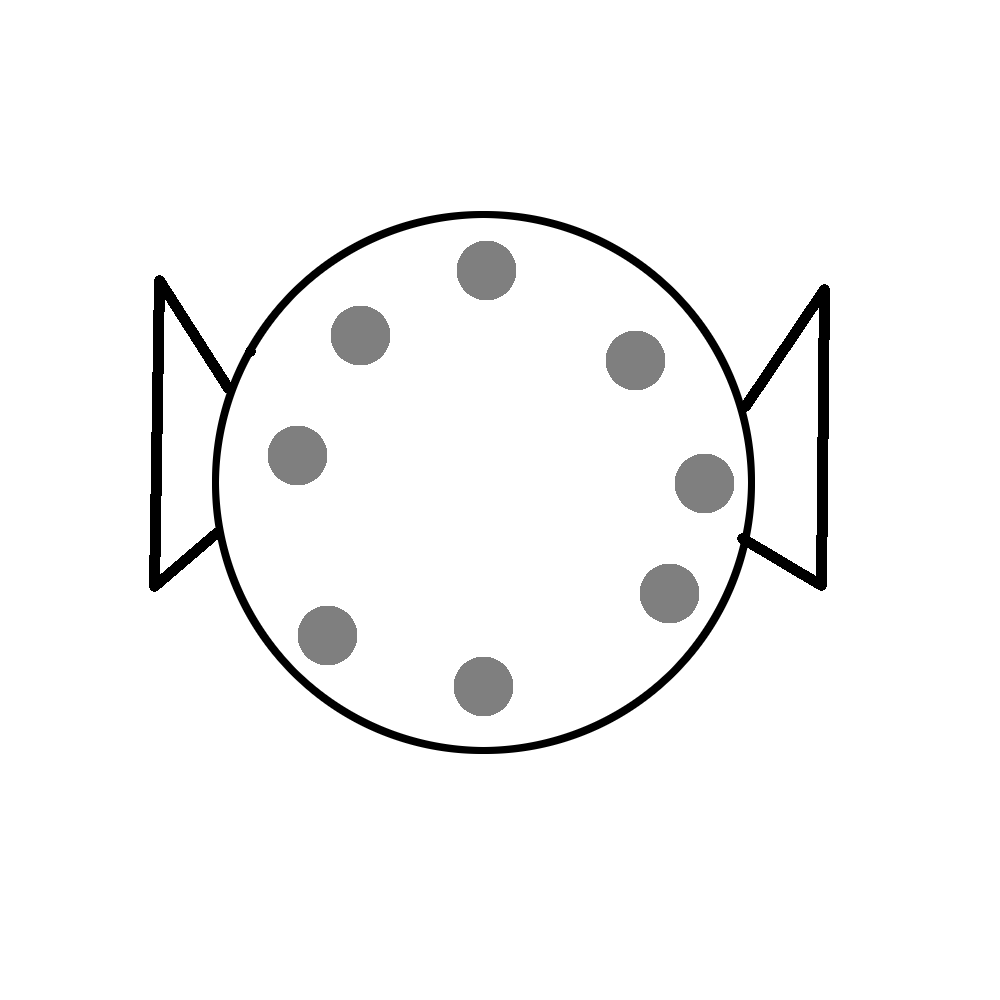
\includegraphics[width=.5\textwidth]{physic1}}%
\only<2>{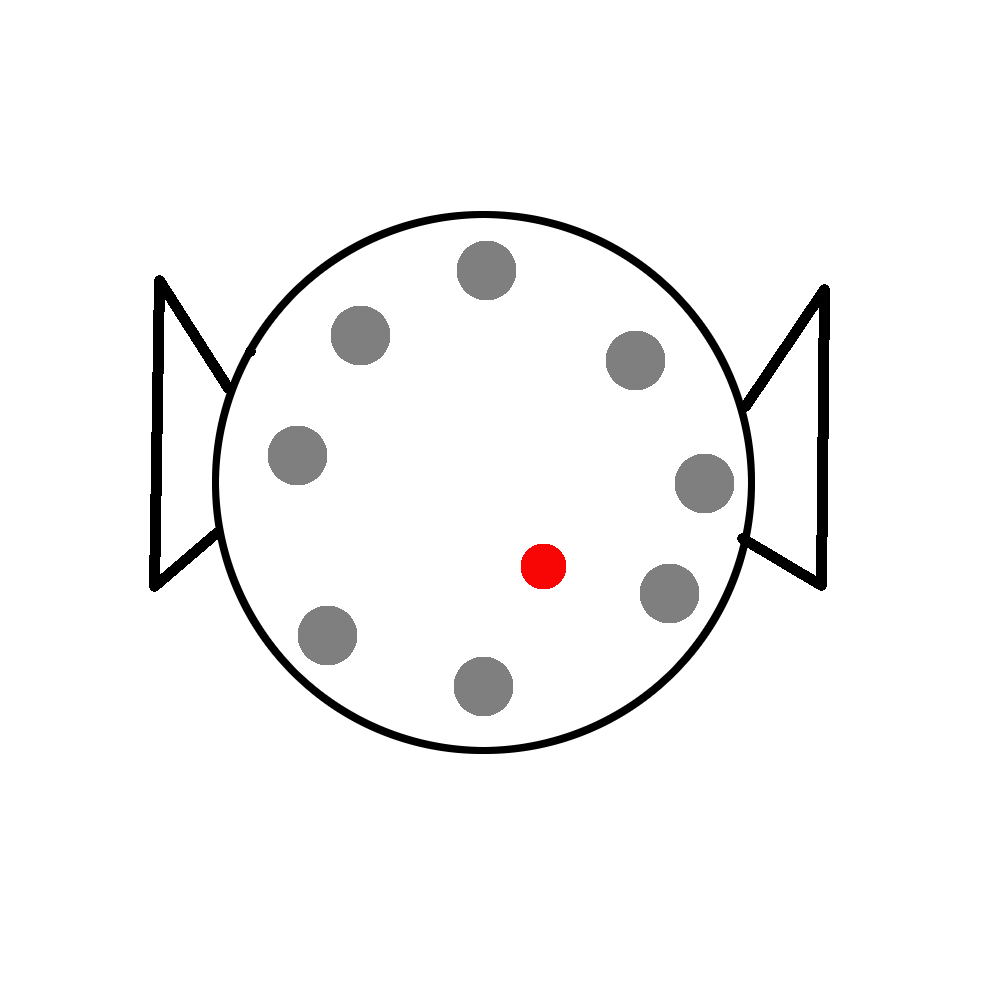
\includegraphics[width=.5\textwidth]{physic2}}%
\only<3>{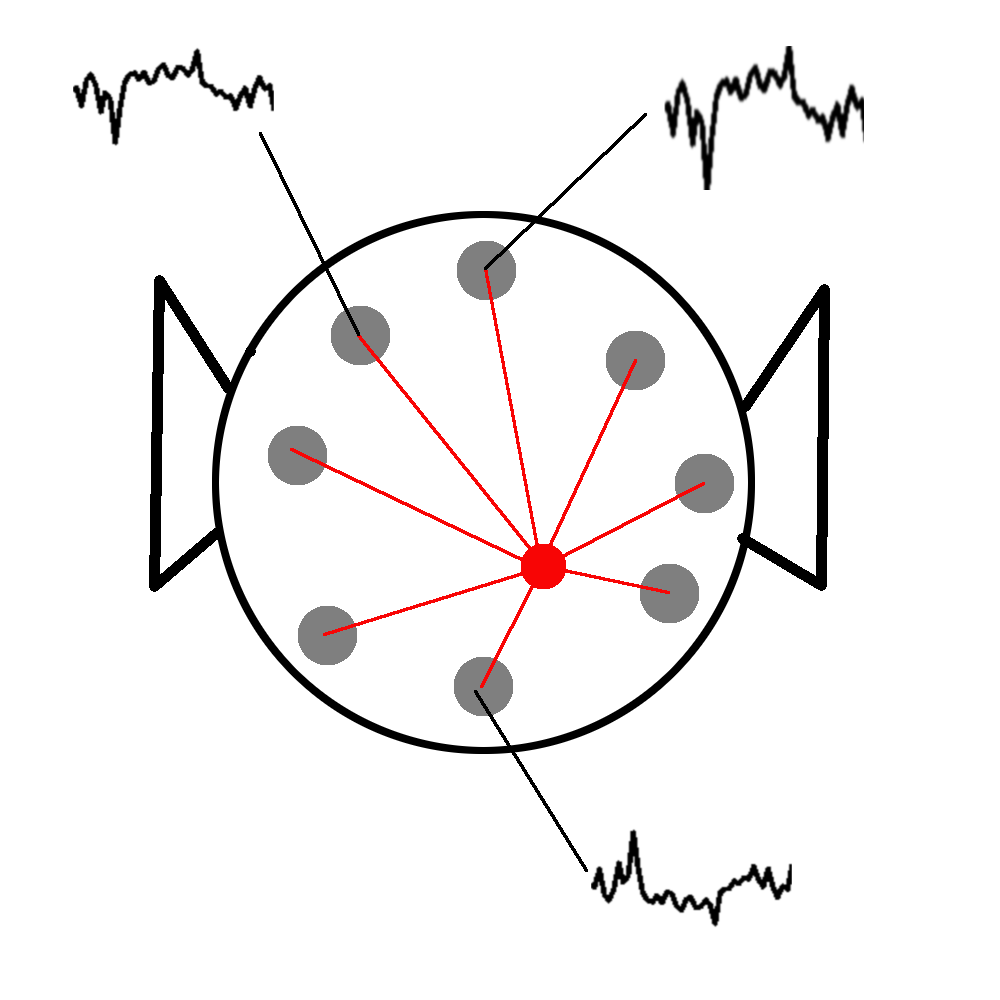
\includegraphics[width=.5\textwidth]{physic3}}%
\only<4>{\vskip1em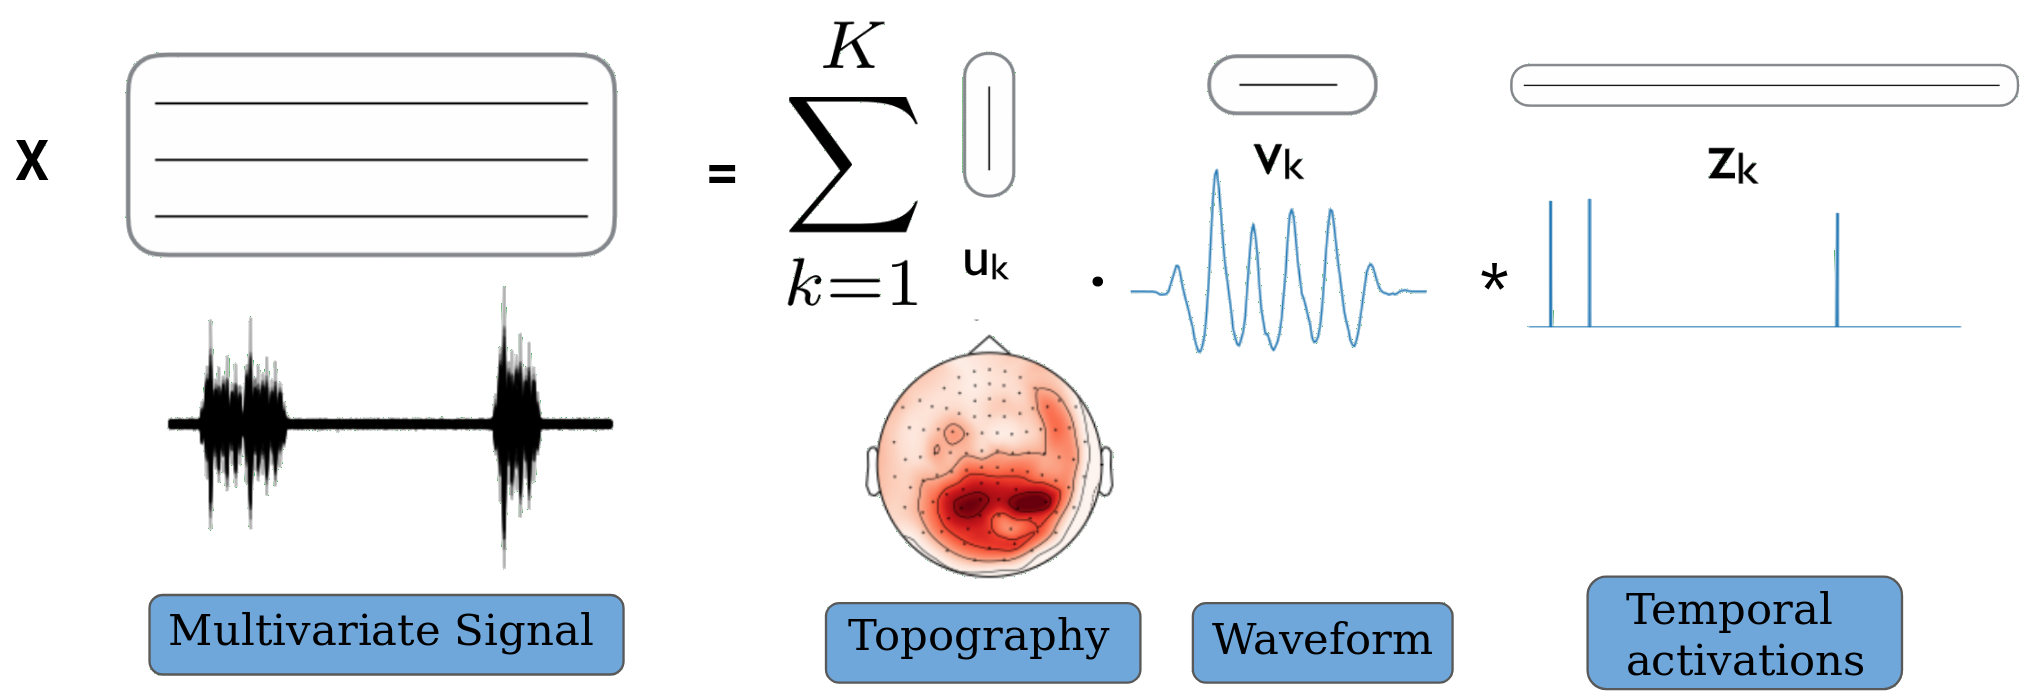
\includegraphics[height=.45\textheight]{rank1}}
\end{frame}

\begin{frame}{Multivariate CSC with rank-1 constraint\\\citeconfright{Dupre2018}{NeurIPS}}
\textbf{Idea}: Impose a rank-1 constraint on the dictionary atoms $D_k$
\vskip1em
To make the problem tractable, we decided to use auxiliary variables $u_k$ and $v_k$ \st{} $D_k = u_kv_k\top$.

\begin{equation}
\label{eq:multichannel_csc}
\begin{split}
\min_{u_k, v_k, z_k^n} &\sum_{n=1}^N\frac{1}{2}\left\|X^n - \sum_{k=1}^K z^n_k * (u_k^{ } v_k^\top)\right\|_{2}^{2}
+ \lambda  \sum_{k=1}^K \left\|z^n_k\right\|_1, \hspace{6pt}\\
&\text{s.t. } ~~ \|u_{k}\|_2^2 \leq 1 \text{  , }\|v_{k}\|_2^2 \leq 1 \text{  and } z_k^n \geq 0~.
\end{split}
\end{equation}

Here,
\begin{itemize}
\item $u_k \in \Rset^P$ is the spatial pattern of our atom
\item $v_k \in \Rset^L$ is the temporal pattern of our atom
\end{itemize}
\strongpoint{Tri-convex optimization problem , solved with alternate minimization.}
\end{frame}


\begin{frame}{Fast optimization}
Comparison with multivariate methods on somato dataset with $T=134,700$, $K=8$, $P=5$ and $L=128$\\[1em]
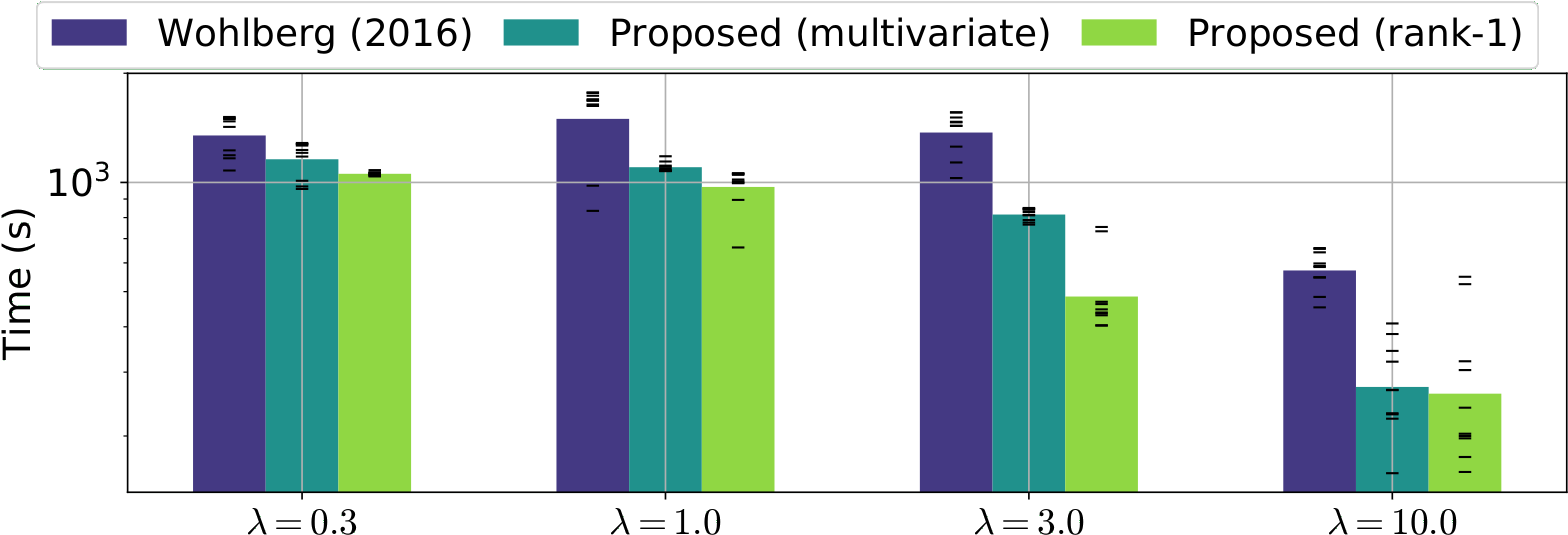
\includegraphics[width=\textwidth]{all_last_0001_T_13470_P5_K8_L128.png}
\end{frame}


%\begin{frame}{Pattern recovery}
%Patterns recovered with $P = 1$ and $P=5$. The signals were generated with the two simulated temporal patterns and with  $\sigma = 10^{-3}$. \\[1em]
%{\centering
%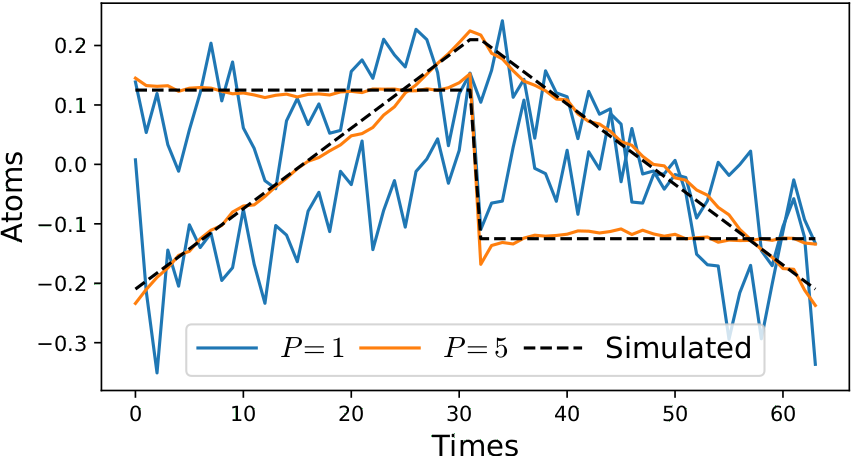
\includegraphics[width=.8\textwidth]{1D_vs_multi_uv_hat_P5.png}\\}
%\end{frame}


\begin{frame}{MNE somatosensory data}
A selection of temporal waveforms of the atoms learned on the MNE sample dataset.\\
\centering
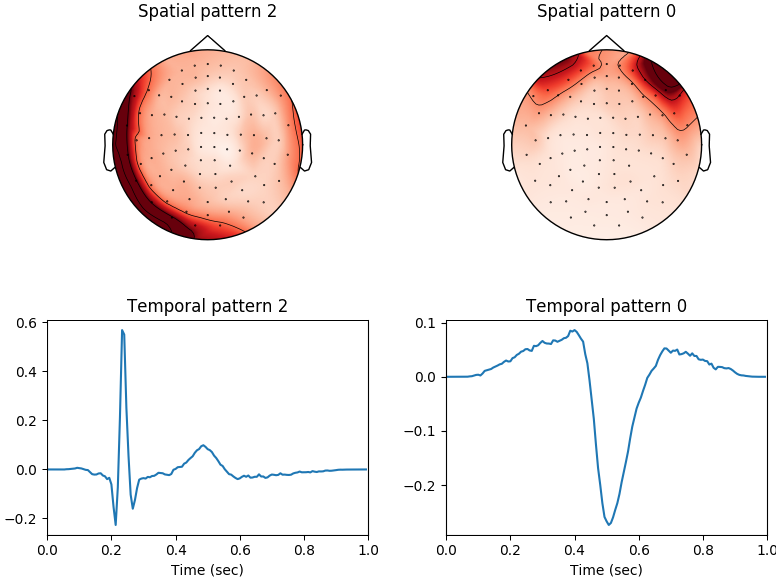
\includegraphics[height=0.8\textheight]{artifacts}
\end{frame}


\begin{frame}{MNE somatosensory data}
Atoms revealed using the MNE somatosensory data. Note the non-sinusoidal comb shape of the mu rhythm.\\[1em]
\centering
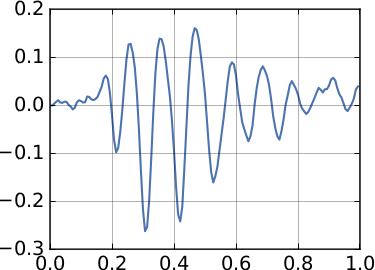
\includegraphics[height=.35\textheight]{atoms_somato_a.png}\hskip3em
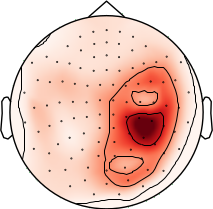
\includegraphics[height=.35\textheight]{atoms_somato_b.png}\\[.3em]\hskip1em
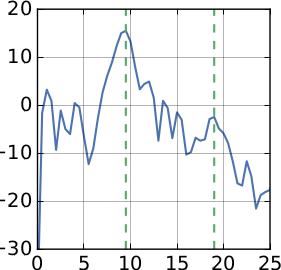
\includegraphics[height=.35\textheight]{atoms_somato_c.png}\hskip3em
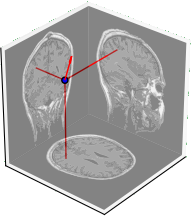
\includegraphics[height=.35\textheight]{atoms_somato_d.png}
\end{frame}



%%%%%%%%%%%%%%%%%%%%%%%%%%%%%%%%%%%%%%%%%%%%%%%%
%   Conclusion
%%%%%%%%%%%%%%%%%%%%%%%%%%%%%%%%%%%%%%%%%%%%%%%%

\begin{frame}{Recap Part III}

\textbf{Take home message}\\[.5em]
\begin{itemize}\itemsep.5em
    \item The structure of the learned dictionary can be constrained to improve the interpretability of the recovered patterns.
    \item Can lead to more efficient algorithm and better recovery property.
    \item Open source package 
\includegraphics[height=.8em]{github}~\url{https://alphacsc.github.io}
\end{itemize}
\vskip1.5em

\textbf{Ahead of us}\\[.5em]
\begin{itemize}\itemsep.5em
    \item Analysis of the patterns learned on large MEG database (HCP).
    \item Link between the learned waveforms and information propagation properties in the brain.
    \item Extension to scale invariant CDL to study frequency coupling in the brain.
\end{itemize}
\end{frame}



\end{document}